\documentclass{beamer}[10]

\usepackage{graphicx}
\usepackage{xcolor}
\usepackage{tabto}
%\usepackage{beamerthemesplit}
\usepackage{tikz}
\usepackage{cancel}
\usepackage{verbatim}
\usepackage{fancybox}
\usepackage{enumerate}
\usepackage{amsmath,amssymb,amsthm,textcomp,mathtools}
\usepackage[super]{nth}
\usepackage[amssymb]{SIunits}
\usepackage{booktabs}
\usepackage{cancel}
\usepackage{bm}
\usepackage[utf8]{inputenc}
\usepackage{tabularx}
\usepackage{ragged2e}
\newcolumntype{Y}{ >{\RaggedRight\arraybackslash}X}
\usetikzlibrary{arrows,shapes}
\newcommand\T{\rule{0pt}{2.6ex}}
\newcommand\B{\rule[-1.2ex]{0pt}{0pt}}
\definecolor{UUcrimson}{RGB}{204,0,0}
\mode<presentation>
{ \usetheme{default}
  \usecolortheme[named=UUcrimson]{structure}
  \useinnertheme{circles}
  \setbeamercovered{transparent}
  \setbeamertemplate{blocks}[rounded]
  \usefonttheme[onlymath]{serif}
  \setbeamertemplate{navigation symbols}{}
  \setbeamertemplate{footline}[page number]
  \setbeamertemplate{navigation symbols}{}
  \setbeamercolor{section in toc}{fg=black,bg=white}
  \setbeamercolor{alerted text}{fg=UUcrimson!80!gray}
  \setbeamercolor*{palette primary}{fg=white,bg=UUcrimson}
  \setbeamercolor*{palette secondary}{fg=UUcrimson!70!black,bg=gray!15!white}
  \setbeamercolor*{palette tertiary}{bg=UUcrimson!80!black,fg=gray!10!white}
  \setbeamercolor*{palette quaternary}{fg=UUcrimson,bg=gray!5!white}
  \setbeamercolor*{palette sidebar primary}{fg=UUcrimson!10!black}
  \setbeamercolor*{palette sidebar secondary}{fg=white}
  \setbeamercolor*{palette sidebar tertiary}{fg=UUcrimson!50!black}
  \setbeamercolor*{palette sidebar quaternary}{fg=gray!10!white}
  \setbeamercolor{titlelike}{parent=palette primary,fg=white}
  \setbeamercolor{frametitle}{bg=UUcrimson}
  \setbeamercolor{frametitle right}{bg=UUcrimson}
  \setbeamercolor*{separation line}{}
  \setbeamercolor*{fine separation line}{}
}

\usetikzlibrary{backgrounds}
\makeatletter
\tikzstyle{every picture}+=[remember picture]
\tikzset{%
  fancy quotes/.style={
    text width=\fq@width pt,
    align=justify,
    inner sep=1em,
    anchor=north west,
    minimum width=\linewidth,
    font=\itshape
  },
  fancy quotes width/.initial={.8\linewidth},
  fancy quotes marks/.style={
    scale=8,
    text=white,
    inner sep=0pt,
  },
  fancy quotes opening/.style={
    fancy quotes marks,
  },
  fancy quotes closing/.style={
    fancy quotes marks,
  },
  fancy quotes background/.style={
    show background rectangle,
    inner frame xsep=0pt,
    background rectangle/.style={
      fill=gray!25,
      rounded corners,
    },
  }
}
\newenvironment{fancyquotes}[1][]{%
\noindent
\tikzpicture[fancy quotes background]
\node[fancy quotes opening,anchor=north west] (fq@ul) at (0,0) {``};
\tikz@scan@one@point\pgfutil@firstofone(fq@ul.east)
\pgfmathsetmacro{\fq@width}{\linewidth - 2*\pgf@x}
\node[fancy quotes,#1] (fq@txt) at (fq@ul.north west) \bgroup}
{\egroup;
\node[overlay,fancy quotes closing,anchor=east] at (fq@txt.south east) {''};
\endtikzpicture}
\makeatother

\usepackage{scalerel}[2014/03/10]
\usepackage{stackengine}
\usepackage{empheq}
\newcommand*\widefbox[1]{\fbox{\hspace{0.5em}#1\hspace{0.5em}}}

\newcommand\reallywidetilde[1]{\ThisStyle{%
  \setbox0=\hbox{$\SavedStyle#1$}%
  \stackengine{-.1\LMpt}{$\SavedStyle#1$}{%
    \stretchto{\scaleto{\SavedStyle\mkern.2mu\sim}{.5467\wd0}}{.4\ht0}%
%    .2mu is the kern imbalance when clipping white space
%    .5467++++ is \ht/[kerned \wd] aspect ratio for \sim glyph
  }{O}{c}{F}{T}{S}%
}}
\usepackage{media9}

\logo{
\includegraphics[width=0.75cm]{logo.jpg}}
\author[Gibbs]{Dr. Jeremy A. Gibbs}
\institute{Department of Mechanical Engineering\\University of Utah}
\date{Fall 2016}
\title{LES of Turbulent Flows: Lecture 24}
\begin{document}

%----------------------------------------------------------------------------------------
%	TITLE & TOC SLIDES
%----------------------------------------------------------------------------------------

\begin{frame} 
  \titlepage
\end{frame}

%------------------------------------------------

\begin{frame}
\frametitle{Overview}
\tableofcontents
\end{frame}

%------------------------------------------------
\section{Special Topic: WALE Model} %
%------------------------------------------------
\begin{frame}{Special Topic: WALE Model}
\begin{itemize}
	\item Recall that many of the LES SGS models we have covered are variants of the eddy-viscosity assumption
	$$\tau_{ij} - \frac{1}{3}\tau_{kk}\delta_{ij} = 2 \nu_T \widetilde{S}_{ij}$$
	where $\nu_T$ is the eddy-viscosity term that must be modeled and 
	$$\widetilde{S}_{ij} = \left(\frac{\partial \widetilde{u}_i}{\partial x_j} + \frac{\partial \widetilde{u}_j}{\partial x_i}\right)$$
	is the strain rate (deformation) tensor of the resolved flow field
\end{itemize}
\end{frame}
%------------------------------------------------
\begin{frame}{Special Topic: WALE Model}
\begin{itemize}
	\item In the case of the Smagorinsky model, we showed that
	$$\nu_T = (C_S \Delta)^2 | \widetilde{S}|$$
	where $\Delta = (\Delta_x \Delta_y \Delta_z)^{\frac{1}{3}}$ is the effective grid scale, $C_S$ is the Smagorinsky coefficient, and 
	$$|\widetilde{S}| = \sqrt{2\widetilde{S}_{ij}\widetilde{S}_{ij}}$$ is the magnitude of the filtered strain rate tensor
\end{itemize}
\end{frame}
%------------------------------------------------
\begin{frame}{Special Topic: WALE Model}
\begin{itemize}
	\item Finally, we showed that if: 
	\begin{enumerate}
		\item we used a spectral cutoff filter,
		\item assume the cutoff wavenumber is in the inertial subrange of a Kolmogorov-type spectrum,
		\item and equate viscous dissipation with the ensemble-average SGS dissipation ($\epsilon = \langle \Pi \rangle$), then
	\end{enumerate}
	$$C_S = \frac{1}{\pi}\left(\frac{2}{3C_k}\right)^{\frac{3}{4}}$$
	where if we assume $C_K \approx 1.4$ we get $$\boxed{C_S \simeq 0.18}$$
\end{itemize}
\end{frame}
%------------------------------------------------
\begin{frame}{Special Topic: WALE Model}
\begin{itemize}
	\item Nicoud and Ducros (1999) challenged the underlying assumption of the Smagorinsky model -- that the local strain rate of the flow defines the velocity scale at the filter width
	\item ND99 also investigated how such a model should behave near the lower boundary (wall)
	\item Additionally, the topic of complex geometry and numerical methods were discussed 
\end{itemize}
\end{frame}
%------------------------------------------------
\begin{frame}{Special Topic: WALE Model}
\begin{itemize}
	\item Recall that $\nu_T$ acts to represent the transfer of energy from resolved to subgrid scales through subgrid dissipation ($\propto \nu_T$)
	\item Accordingly, using the Smagorinsky-style model, the subgrid dissipation is described by the strain rate of the smallest resolved scales
	\item However, Wray and Hunt (1989) showed from DNS of isotropic turbulence that energy is actually concentrated around zones of vorticity and strain
	\item Thus, using only the strain rate is inadequate
\end{itemize}
\end{frame}
%------------------------------------------------
\begin{frame}{Special Topic: WALE Model}
\begin{itemize}
	\item ND99 suggested a better SGS model would account for both strain rate and rotational rate
	\item One example is an eddy-viscosity model based on the structure function
	$$\nu_T = \beta C_k^{-3/2} \Delta \sqrt{\widetilde{F_2}}$$
	where $\widetilde{F_2}$ is the second-order velocity structure function of the filtered field
	$$\widetilde{F_2}(\vec{x},\Delta) = \langle |\widetilde{\vec{u}}(\vec{x}+\vec{r},t) - \widetilde{\vec{u}}(\vec{x},t)|^2\rangle$$
	and $\beta$ is a constant (Lesieur and Metais 1999 suggested $\beta = 0.105$ for isotropic turbulence)
\end{itemize}
\end{frame}
%------------------------------------------------
\begin{frame}{Special Topic: WALE Model}
\begin{itemize}
	\item Another issue beyond the physical description of the model is how it behaves near the wall
	\item The Smagorinsky model will give non-zero values of $\nu_T$ provided gradients exist -- however in the reality turbulent fluctuations are damped near the wall so that $\nu_T$ should be zero
	\item One way to correct this in the past was the Van Driest exponential damping function
	$$1 - exp({-y^+/A^+}) \qquad \text{where } A^+ = 25$$
	\item Recall from Lecture 14 that Deardorff also implemented an enhancement of dissipation near the wall to prevent unnatural build-up of energy
\end{itemize}
\end{frame}

%------------------------------------------------
\begin{frame}{Special Topic: WALE Model}
\begin{itemize}
	\item While these damping methods improve results, they are \textit{ad hoc} and are difficult to apply to complex geometries
	\item ND99 notes that there are ways to try and force near-zero $\nu_T$, which includes limiting the distance over which $\widetilde{F_2}$ is computed, or computing $C_S$ dynamically (as in Germano)
	\item Recall, however, that the dynamic procedure may result in a large fraction of negative $C_S$ values, which can lead to numerical instability
	\item While spatial averaging can alleviate this problem, the required size of the stencil is not really known \textit{a priori}, it is \textit{ad hoc}, and it is limited to simple flow geometries
\end{itemize}
\end{frame}

%------------------------------------------------
\begin{frame}{Special Topic: WALE Model}
\begin{itemize}
	\item The general form of these models can be given by
	$$\nu_T = C_m \Delta^2 \widetilde{OP}(\vec{x},t)$$
	where $C_m$ is the model coefficient and $\widetilde{OP}$ is an operator defined from the resolved scales
	\item ND99 proposed a new operator with the following properties
	\begin{itemize}
	\item invariant to coordinate rotation or translation
	\item easily assessed on any computational grid
	\item function of both strain and rotation rates
	\item goes naturally to 0 at the wall
	\end{itemize}
	\item Called the Wall-Adapting Local Eddy-viscosity (WALE) model
\end{itemize}
\end{frame}
%------------------------------------------------
\begin{frame}{Special Topic: WALE Model}
\begin{itemize}
	\item $\widetilde{OP}$ must be based on invariants of a tensor $\tau_{ij}$, which represents turbulence
	\item Velocity gradient tensor $(\widetilde{g}_{ij} = \partial \widetilde{u}_i / \partial x_j)$ is a good candidate
	\item Smagorinsky was based on second invariant of the symmetric part of $\widetilde{S}_{ij}$ of this tensor (see Lecture 7)
	\item Two drawbacks with Smagorinsky approach: \\1.) only considers strain rate of structures, not rotational rate \\2.) leads to unphysical $\nu_T = \mathcal{O}(1)$ at the surface 
\end{itemize}
\end{frame}

%------------------------------------------------
\begin{frame}{Special Topic: WALE Model}
\begin{itemize}
	\item ND99 constructed a new proposed (and hopefully better) operator by considering the traceless symmetric part of the square of the velocity gradient tensor
	$$S_{ij}^d = \frac{1}{2}\left(\widetilde{g}^2_{ij} + \widetilde{g}^2_{ji}\right) - \frac{1}{3}\delta_{ij} \widetilde{g}^2_{kk}$$
	where $\widetilde{g}^2_{ij} = \widetilde{g}_{ik}\widetilde{g}_{kj}$
	\item Note: the antisymmetric part of $\overline{g}$ is given by
	$$\widetilde{\Omega}_{ij} = \frac{1}{2} \left( \frac{\partial \widetilde{u}_i}{\partial x_j} + \frac{\partial \widetilde{u}_j}{\partial x_i}\right)$$
\end{itemize}
\end{frame}
%------------------------------------------------
\begin{frame}{Special Topic: WALE Model}
\begin{itemize}
	\item After some math (see ND99 on Canvas or website), the WALE model is given by
	$$\nu_T = (C_w\Delta)^2 \frac{ \left( S_{ij}^d S_{ij}^d \right)^{3/2}}{\left( \widetilde{S}_{ij} \widetilde{S}_{ij} \right)^{5/2} + \left( S_{ij}^d S_{ij}^d \right)^{5/4}}$$
	where
	$$C_w^2 = C_S^2 \frac{ \left\langle \sqrt{2}\left(\widetilde{S}_{ij} \widetilde{S}_{ij}\right)^{3/2}\right\rangle}{ \left\langle \widetilde{S}_{ij} \widetilde{S}_{ij} \left( S_{ij}^d S_{ij}^d \right)^{3/2} \left( \left( \widetilde{S}_{ij} \widetilde{S}_{ij} \right)^{5/2} + \left( S_{ij}^d S_{ij}^d \right)^{5/4} \right)^{-1} \right\rangle}$$
	For $C_S\approx0.18$, expect $0.55 \leq C_w \leq 0.60$ 
\end{itemize}
\end{frame}
%------------------------------------------------
\begin{frame}{Special Topic: WALE Model}
\begin{itemize}
	\item The WALE model formulation accounts for rotational rate, naturally goes to 0 at the wall without the need for any \textit{ad hoc} methods, and can be generalized for any grid and complex geometries
\end{itemize}
\end{frame}
%------------------------------------------------
\begin{frame}{Special Topic: WALE Model}
\begin{itemize}
	\item One first test was to see how well the WALE model produced spectra for decaying isotropic turbulence
	\begin{figure}
		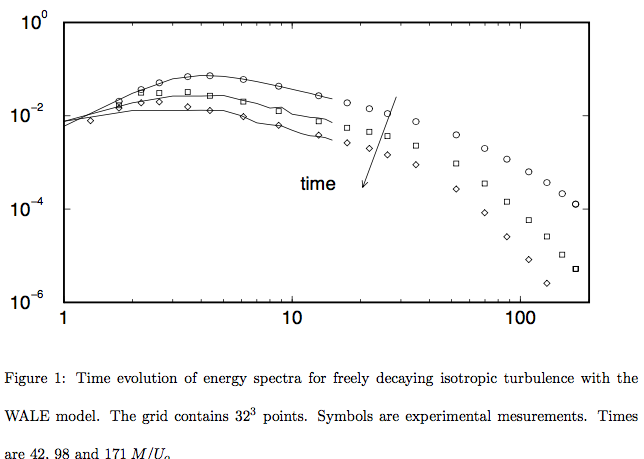
\includegraphics[width=0.8\textwidth]{wale1}
	\end{figure}
\end{itemize}
\end{frame}
%------------------------------------------------
\begin{frame}{Special Topic: WALE Model}
\begin{itemize}
	\item In the next test ND99 examined the WALE model in a turbulent pipe flow using a hybrid grid
	\begin{figure}
		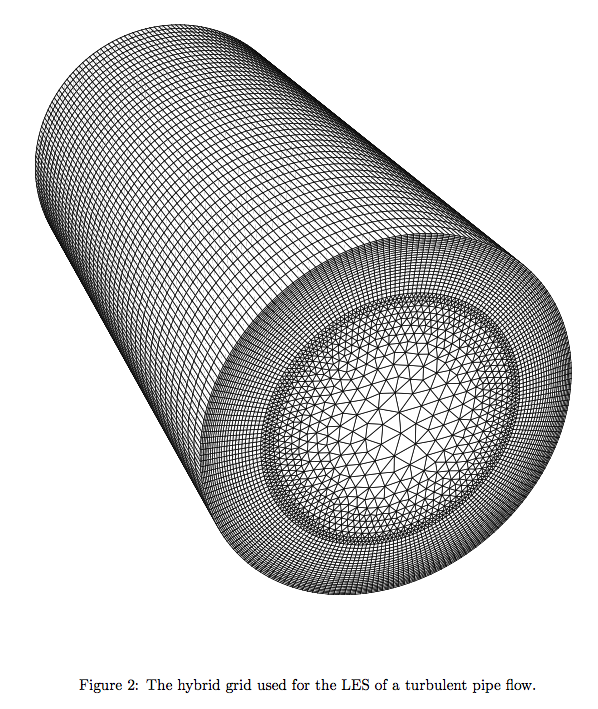
\includegraphics[width=0.55\textwidth]{wale2}
	\end{figure}
\end{itemize}
\end{frame}
%------------------------------------------------
\begin{frame}{Special Topic: WALE Model}
\begin{itemize}
	\item Results from turbulent pipe flow tests
	\begin{figure}
		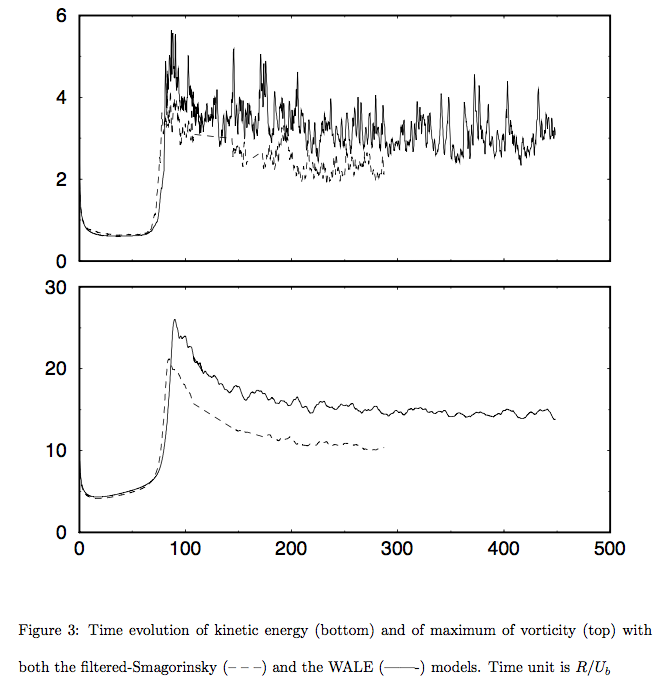
\includegraphics[width=0.65\textwidth]{wale3}
	\end{figure}
\end{itemize}
\end{frame}
%------------------------------------------------
\begin{frame}{Special Topic: WALE Model}
\begin{itemize}
	\item Results from turbulent pipe flow tests
	\begin{figure}
		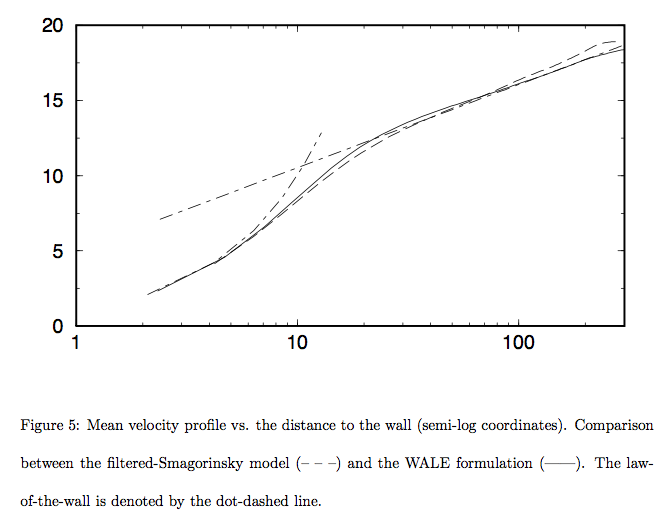
\includegraphics[width=0.75\textwidth]{wale4}
	\end{figure}
\end{itemize}
\end{frame}
%------------------------------------------------
\begin{frame}{Special Topic: WALE Model}
\begin{itemize}
	\item Results from turbulent pipe flow tests
	\begin{figure}
		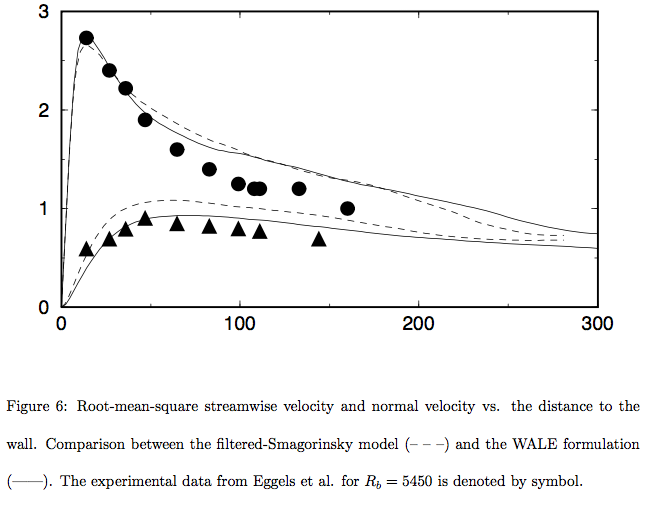
\includegraphics[width=0.75\textwidth]{wale5}
	\end{figure}
\end{itemize}
\end{frame}


%------------------------------------------------


\end{document}

